\section{Exploring Inward-Directed Photon Emission Using Radio Polarization Data of PSR J1057$-$5226}

\paperref{This section is based on work done for
``Exploring Inward-Directed Photon Emission Using Radio Polarization Data of PSR J1057$-$5226''}



We apply a bidirectional model with both outward-directed photons
and inward-directed photons to understand the complex
radio polarization data of PSR J1057$-$5226 (PSR B1055$-$52).
PSR J1057$-$5226 radio polarization data matches well to
this model  when one of the
components of the polarization sweep is associated with
inward-directed photon emission.
Additionally, we discuss previous studies
of PSR J1057$-$5226 in relation to our current study
and past applications of models with inward-directed photons.
We apply $\gamma$-ray models restricted by best fit parameters
from the radio modeling.  Although possible solutions exist, results
do suggest we have not fully identified the
location of the emission within the magnetosphere with the
simplest $\gamma$-ray modeling assumptions.


\subsection{Introduction}

Pulsars have strong magnetic fields that are tied fundamentally to the
emission observed from Earth.  Charged particles follow the magnetic
field lines before emitting curvature radiation.  The projected
position angle of such radiation is a means of observing directly
the geometry of the pulsar magnetic field and is a powerful
tool for understanding the magnetosphere and the emission
mechanism of the pulsar.

A large number of pulsars have S-shaped polarization
position angle sweeps (versus phase).
A simple analytical formula which assumes the pulsar
is a vacuum point dipole
predicts these S-shaped sweeps.
This model
is called the rotating vector model (RVM, \citealp{radhakrishnan1969magnetic}).
Given the simplicity of
the model, it works surprisingly well for quite a number of
pulsar position angle data sets
(i.e. \citealp{lyne1988shape}, \citealp{phillips1990magnetic}, \citealp{everett2001emission}).

Nevertheless, for other pulsars, the polarization does not
adhere to this smooth S-shape form and has jumps and cusps that
fundamentally can not be explained using such a simple model
(i.e. \citealp{yan2011polarization}, \citealp{everett2001emission}).
Few studies have attempted to understand in-depth this difficult data but
polarization is a powerful tool for understanding
the emission of pulsars even for ``messy'' radio polarization sweeps.
Further, pulsars with complex polarization tend to be high energy
pulsars seen in the $\gamma$-rays and thus understanding these
complicated polarization sweeps will contribute to understanding 
pulsars in multi-wavelength studies (e.g. \citealp{keith2012high}).
Overall, 
developing models for this complicated
and little understood polarization
has great potential for elucidating the geometry and
emission of the pulsars.

In a previous paper (\citealp{craig2014tackling}), our aim was to build on the
simple rotating vector model (RVM).  We numerically calculated
polarization from finite altitude with and without
orthogonal mode jumps \citep{backer1976orthogonal}.
RVM accurately predicts only emission from 
the surface of the point neutron star, an altitude of zero,
because of the lack of relativistic considerations. 
The addition of finite altitude also allows for multiple-altitude
models with emission from multiple areas in the pulsar magnetosphere.
The addition of multiple altitudes explains well a number
of the jumps seen in the complex polarization data.  (A jump
in a polarization sweep for example can be seen in Figure~\ref{fig:singleAlt} 
between the polarization associated with intensity peaks $C_2$ and $C_3$.)

In \cite{craig2014tackling}, we illustrated our model by fitting 
the model to a number of pulsars.  One of these pulsars was PSR J1057$-$5226.
The polarization of the trailing component of the
$P_1$ pulse (labeled as $C_3$ in Figure~\ref{fig:singleAlt}) 
which appears to have a jump in the polarization when compared
to the rest of the sweep was not modeled.  In this current paper, this component
is treated as ``backward'' emission.
In adhering to a modified geometrically based model, this
inward-directed photon emission is calculated using the field lines of the
typical dipole but aimed in the opposite direction
of the typical outward-directed photon.  The addition of 
polarization from inward-directed photon emission is the natural next step for
a model based on geometry and guided by data.

In this current paper, we will fit the pulsar radio
polarization data and  $\gamma$-ray data and argue that
PSR J1057$-$5226 has atypical emission that makes it
a particularly interesting candidate for inward-directed photon emission.
Figure~\ref{fig:simpleFig} illustrates the configuration of 
pulsar PSR J1057$-$5226 with bidirectional photon emission.
We will discuss the formal fitting of the polarization data for PSR J1057$-$5226
in Section \ref{sec:fitting} along with fitting of the $\gamma$-ray data. 
In Section \ref{sec:intro}, we review past studies on PSR J1057$-$5226.
In Section \ref{sec:previousBidirectional}, we review
previous studies that consider bidirectional emission.

\begin{figure}[t!!]
\begin{center}
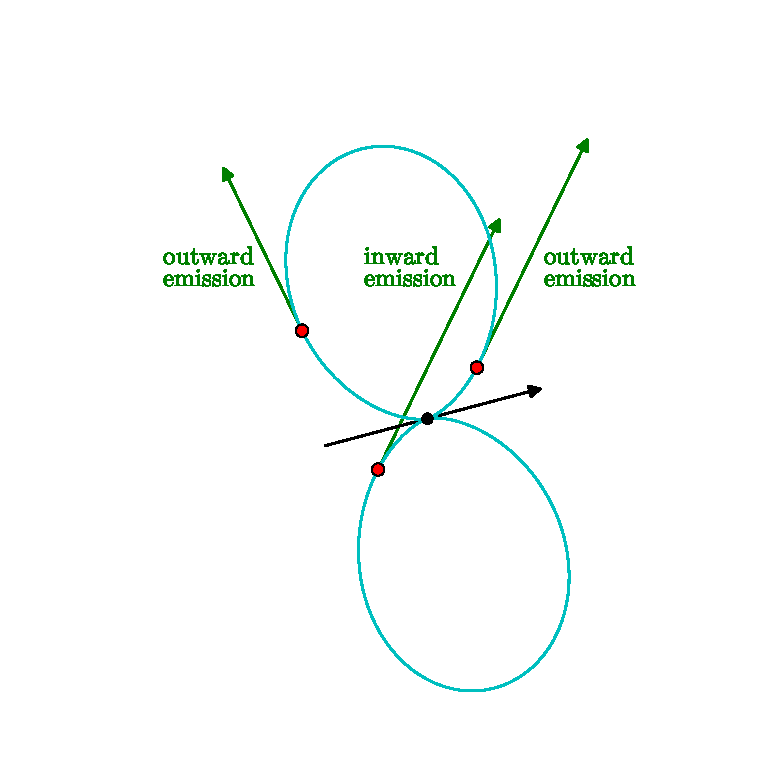
\includegraphics[scale=.8]{chapters/inwardDirectedPhotons/figures/magnetosphere.eps}
\caption[Sketch of a pulsar magnetosphere illustrating the use of inward-directed photon
emission to explain unusual polarization of PSR J1057$-$5226]{\label{fig:simpleFig}
Sketch of a pulsar magnetosphere illustrating the use of inward-directed photon
emission to explain unusual polarization of PSR J1057$-$5226. The rotation axis is
vertical. Green lines are emission from various regions of the magnetosphere
originating at red dots. Two regions emit the typical outward-directed photons
and another region emits inward-directed photons. All three arrows have the
same line of sight angle from the spin axis and thus all three will be seen by
a single observer. In terms of phase, the observer will see emission from
the ``outward'' emission on the right side of the diagram followed
quickly by the ``inward'' emission for a counter-clockwise spinning
pulsar. The pulsar will then swing around and the ``outward'' emission
on the left side of the diagram will be in the line of sight of the observer.
Thus the observer will see two pulses in the pulsar emission although one of
the pulses contains both inward-directed photons and outward-directed photons
each from a separate pole. This configuration is the one that is supported
by polarization data for PSR J1057$-$5226 and the diagram is a simplified version of Figure~\ref{fig:totDirFitPhi}.
}
\end{center}
\end{figure}



\subsection{Previous Work with PSR J1057$-$5226}
\label{sec:intro}



The pulsar PSR J1057$-$5226 (also known as PSR B1055$-$52) is a relatively young pulsar
($P=197.11$ms) with emission in the radio and $\gamma$-rays.  In radio, PSR J1057$-$5226 exhibits two
pulses with an approximate 180$^\circ$ separation in phase.  The $\gamma$-rays have been studied
using the outer gap and the two-pole caustic models (\citealp{romani2010constraining}).  
\cite{weltevrede2009mapping} have studied PSR J1057$-$5226 in radio; they applied
the RVM to the radio position angle polarization data and
applied opening angle arguments to map the polar cap emission region.  With these
models, they were forced to conclude that some emission originates from field lines outside 
the formal dipole open zone cap.  This cap is defined by field lines on the
neutron star surface that extend outside of the
light cylinder (characterized by a cylindrical distance, $R_{\rm{LC}}$, at which particles
would have to travel faster than the speed of light to co-rotate) and do not close.
They also
applied the analytic Blaskiewicz, Cordes, Wasserman (BCW, \citealp{blaskiewicz1991relativistic})
formulation to approximate different altitudes for the two pulses of 
emission.



In a previous paper (\citealp{craig2014tackling}), we applied 
a numerical geometrically-based model to an updated polarization
position angle sweep of PSR J1057$-$5226. 
Such a model 
can accurately produce polarization sweeps of much greater
heights  than the
simplistic BCW formulation. \cite{craig2012altitude}
calculated break-down altitudes to be $\sim0.05\rm{-}0.12R_{\rm{LC}}$
for BCW (depending on geometric parameters and intensity models).
The data could be modeled with emission originating mostly 
from within the open zone of the magnetosphere but at
altitudes near the formal light cylinder.  The data could
also be modeled at lower altitudes with emission originating
from well within the closed zone of the magnetosphere.

Additionally, the updated polarization position angle data used in \cite{craig2014tackling}
revealed an additional piece of polarization previously not noted in \cite{weltevrede2009mapping}.
In \cite{craig2014tackling}, we were unable to fit this piece of polarization even 
with multiple altitudes and orthogonal mode jumps (\citealp{backer1976orthogonal}).  

\cite{weltevrede2012phase}, a follow-up paper to \cite{weltevrede2009mapping}, has a 
detailed analysis of the periodic modulation of PSR J1057$-$5226. 
They found that for the $20$ period modulation, the two pulses of PSR J1057$-$5226 have a $2.5$ period phase-locked delay.
If the two pulses originate from separate poles, this delay can not be easily or simply 
explained.  Either there must be some form of communication between the poles, the emission originates
from a single pole, or some external factors are at play.
See \cite{weltevrede2012phase} for a discussion summarizing these possibilities.  


\subsection{Previous Work in Bidirectional Emission}
\label{sec:previousBidirectional}

Bidirectional emission was suggested
for pulsar radio emission in general by \cite{dyks2005reversals}.
Bidirectional emission is emission with both an outward-directed photon component
and an inward-directed photon component and is 
also called
backward or downward emission.
The inward-directed emission originates from
one pole but instead of being directed outward from the neutron star,
it is directed into the typical cone of emission and is therefore seen
at a phase that one would expect emission from the opposite
pole.  
In recent years, bidirectional emission has been suggested for 
a number of pulsars.

Figure~\ref{fig:simpleFig} offers a visual representation of bidirectional emission. In the
figure, the black arrow is the magnetic axis, the cyan loops are a pair of
field lines, and the rotation axis is vertical (not shown). The red points
represent regions where emission is produced and the green arrows represent
the path of a photon traveling tangent to the field line. All three emission
projections marked by the green arrows will be visible to a single observer
during the rotation of the pulsar. The ``outward'' emission will be
seen as the typical two pulses of the pulsar. The ``inward'' emission
will be seen near in phase to the ``outward'' emission on right side of
the diagram even though this ``inward'' emission originates from the
opposite pole.


\cite{dyks2005reversals} argued for bidirectional emission in the pulsar PSR B1822$-$09.
The interpole component of the pulsar radio profile disappears when the precursor 
component of the main pole emission appears and vice versa \citep{gil1994multifrequency}.
This behavior suggests some interpole communication or perhaps bidirectional
behavior.  In \cite{dyks2005reversals}, they estimated the radial distance of the emission
based on phase lag between the inward-directed and outward-directed photon emission assuming
both emission components come from the same region. They also estimated $\alpha$
(angle between rotation axis and magnetic axis)
based on observing both components.  Further, they argue that 
inward-directed photon emission components are more common than recognized because one does not always
see both inward-directed and outward-directed photon emission components but only the nulling of the visible 
component.

PSR B0950$+$08, PSR B1929$+$10, and PSR B0437$-$4715 were suggested to have bidirectional emission by 
\cite{dyks2005shadow}.  These three pulsars are so-called ``notched" pulsars \citep{mclaughlin2004notches}
because in radio intensity two notches of emission appear on the leading side of the main pulse,
one partially embedded in the main pulse and the other several degrees before the main
pulse.  \cite{wright2004model} argued for a model where a obscuration in the magnetosphere
along with multiple altitudes causes the double notch emission.  \cite{dyks2005shadow} created
a model where inward-directed photons are the source of this emission and the pulsar
itself is the obstruction.  In later papers however, they favor other models
to explain the double notches \citep{dyks2006model,dyks2012asymmetry}.

In \cite{weltevrede2007main}, the interaction of the two pulses of PSR B1702$-$19 is explored.  The pulsar radio intensity 
periodically brightened every 10.4 periods.  The main pulse modulation lags the interpulse modulation
by 0.43 periods.  One explanation for this phase-locked behavior is bidirectional emission where the
interpole component actually originates from inward-directed photon emission in the same region of the magnetosphere as the
outward-directed photon emission of the main pulse.  In the paper, the authors also discuss other possible explanations
such as a single wide pole.  They also discuss possible geometrical configurations needed for
bidirectional emission in PSR J1057$-$5226 and PSR B1822$-$09 based on observed
periodic intensity modulations of these pulsars.  

\cite{weltevrede2012interpole} found that the pulsar PSR J1057$-$5226 has 
a phase-locked
delay of $2.5$ periods between the pulses for the observed modulations
that occur every $20$ periods.
As pointed out in \cite{weltevrede2012interpole}, a phase-locked
delay of $2.5$ periods for the pulsar PSR J1057$-$5226 is far too long to be simply explained by the time-of-flight
delay of bidirectional emission.  But as pointed out in \cite{weltevrede2012phase}
such a delay could be caused by magnetospheric reflection or drift
(\citealp{wright2003empirical} and \citealp{melrose2012obliquely}).
We discuss this further in Section~\ref{sec:comp2012}.

\subsection{Modeling Data of PSR J1057$-$5226}
\label{sec:fitting}

\begin{figure*}[htbp]
\vskip .041\textheight
\begin{center}
%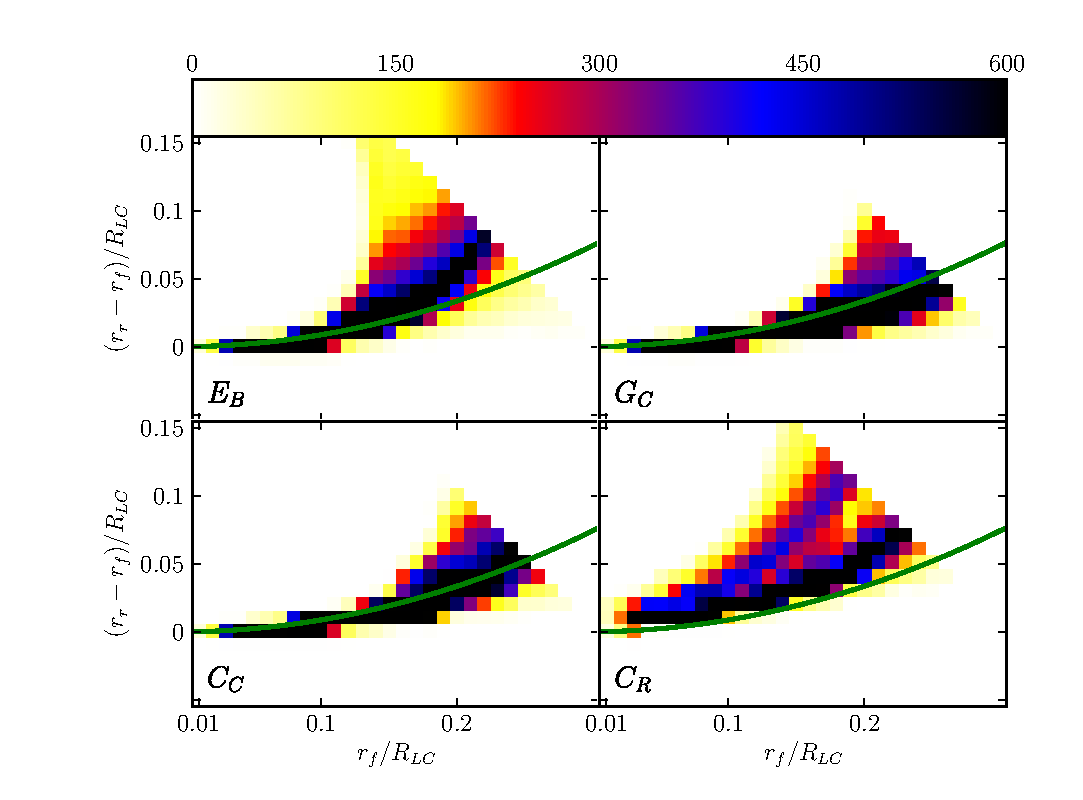
\includegraphics[width=.7\textwidth]{chapter2figures/totDirFitPhi.eps}
\special{psfile=chapters/inwardDirectedPhotons/figures/test2.eps hoffset=-145 voffset=-361 vscale=71 hscale=71}
%\special{psfile=testCloseUp.eps hoffset=-140 voffset=-395 vscale=75 hscale=75}
\begin{flushright}

\begin{overpic}[width=.66\textwidth]{chapters/inwardDirectedPhotons/figures/testCloseUp3a.eps}
\multiput(-10,30.5)(.8,-.65){30}
{\line(2,0){0.5}}
\multiput(-9.5,40.4)(.8,.44){30}
{\line(2,0){0.5}}
\end{overpic}

%\includegraphics[width=.66\textwidth]{testCloseUp2.eps}
\end{flushright}
%\special{psfile=testCloseUp.eps hoffset=100 voffset=-50 vscale=100 hscale=100}
\caption[Visualization of the pulsar model at parameters for
which $\chi^2$ is minimized assuming a single altitude of 
bidirectional emission for PSR J1057$-$5226]{
The left panel shows a visualization of the pulsar model at parameters for 
which $\chi^2$ is minimized assuming a single altitude of bidirectional emission
for PSR J1057$-$5226.  
The symbols $C_1/C_2$, $C_3$, and $P_2$ label the geometrical 
emission sites of various
polarization position angle sweep pieces 
as seen in Figure~\ref{fig:singleAlt}.
The regions $C_1/C_2$ and $P_2$ are assumed to originate
from outward-directed photons on opposite poles while
$C_3$ originates from inward-directed photons on the same pole
as $P_2$.
For this particular model
$\alpha=77^\circ$.  The cyan magnetic field lines are the last closed field
lines with $\rho_{\rm{ypt}}=0.45R_{\rm{LC}}$ and the yellow magnetic field lines are
the last closed field lines with $\rho_{\rm ypt}=1R_{\rm{LC}}$.  The red
lines and green arrows highlight regions of emission seen for $\zeta=44^\circ$
and $R_{C_1/C_2}=R_{C_3}=R_{P_2}=0.35R_{\rm{LC}}$, the best fit configuration for a single-altitude model.   The right panel is a close up of the 
pulsar with fewer magnetic field lines (yellow and cyan lines).  The transparent caps represent
regions of open field lines at $R=0.35R_{\rm{LC}}$ and $\rho_{\rm{ypt}}=0.45R_{\rm{LC}}$.
The region enclosed in the thin black line on the caps represent 
the region of open field lines with $\rho_{\rm{ypt}}=1R_{\rm{LC}}$ 
(the classical vacuum cap).  Thick curved red lines on the caps represent
regions from which we do see emission while thin curved red lines are regions
that we could see emission from for $\zeta=44^\circ$.  The rotation
axis is vertical. 
}
\label{fig:totDirFitPhi}
\end{center}
\vskip .02\textheight
\end{figure*}



\subsubsection{Fitting Procedure for Polarization Position Angle Data}
\label{sec:fitProcedure}
The model used in this paper is the same finite-altitude (measured radially from the neutron star center),
geometrically-based model as used in \cite{craig2014tackling}.
\cite{craig2014tackling} contains a more detailed description
of the model and its nuances.
The allowed range of fit altitude was  $R=R_{\rm{NS}}$ to $0.9R_{\rm{LC}}$
where $R_{\rm{NS}}$ is the neutron star radius for PSR J1057$-$5226.
The angles $\alpha$, the angle between the spin axis and
magnetic axis, and $\zeta$, the viewing angle measured from 
the spin axis were held fixed in $1^\circ$ intervals while 
all other parameters varied.  The other fit parameters
were the horizontal and vertical offsets ($\Delta \phi$ 
and $\Delta \psi$) and the altitudes ($R_{C_1/C_2}$, $R_{C_3}$, and $R_{P_2}$).
The parameters $\Delta \phi$ and $\Delta \psi$
shift the polarization position data relative to the model horizontally
and vertically.
Although these parameters contain important physical information
(the phase of closest approach of the magnetic axis and 
the absolute position angle of the magnetic axis on the
plane of the sky), they are not reported here and are treated more as 
nuisance parameters.
Additionally, phase of zero in the radio polarization
model is the same as phase of zero in the $\gamma$-ray model
(see Section \ref{sec:gam}).
The altitudes are measured radially from the center of the pulsar and
are the distance at which photons are emitted tangent to the magnetic 
field lines.  The magnetic field line structure used here is 
that of a relativistic rotating point dipole given in \cite{kaburaki1980determination}.
A simulated annealing scheme was used to minimize
$\chi^2$ \citep{flannery1992numerical} and to randomly sample
the fit parameter space within $3\sigma$  of the $\chi^2_{\rm{min}}$
and calculate fit error bars.  We also
allowed for orthogonal mode jumps.

In this paper, as in \cite{craig2014tackling}, we use the parameter
$\rho_{\rm{ypt}}$.  This parameter is the cylindrical distance
required of the last closed field line (or the y-point)
for all emission seen in the data to originate from
open field lines. For the classical vacuum dipole 
model, $\rho_{\rm{ypt}}=1R_{\rm{LC}}$.  In terms of emission
phase, the smaller the $\rho_{\rm{ypt}}$, the more
time or phase an observer should see signal from the
pulsar for any given pulsar configuration.

We will also refer to the value $\Delta\rho=\rho_{\rm{ypt}}-\rho_{\rm{max}}$.
The value $\rho_{\rm{max}}$ is the maximum cylindrical distance 
of the model emission
from the neutron star
center (the maximum cylindrical altitude of the model;
whereas, $R_{C_1/C_2}$, $R_{C_3}$, and $R_{P_2}$ are radial distances).  

In modeling PSR J1057-5226 data, we assume that radio emission identified as $C_1$ and $C_2$ in
Figure~\ref{fig:singleAlt} originates from the ``main pulse''
pole of the pulsar. 
Here the main pulse pole is the one that has the
closest approach to the observer. The ``interpulse'' pole is then the
pole from which the emission identified as $C_3$ and $P_2$ originates. This
definition is contrary to the one used in \cite{weltevrede2009mapping} in which the
pulse labeled as $P_1$ in the current paper is the ``interpulse'' and $P_2$
is the ``main pulse''. The pulse $P_2$ was likely chosen as the
``main pulse'' because it contains the peak of largest intensity. Also
note that \cite{weltevrede2009mapping} used a different geometric angle
convention from the current paper and must be converted to make direct
comparisons. See \cite{everett2001emission} for an explanation and the
conversion formula.

We fit the polarization data for PSR J1057$-$5226 assuming that (1) the altitude 
for all three components (outward-directed photon emission component from the main pulse, outward-directed photon emission component from the interpulse, 
and inward-directed photon emission component from the interpulse) are different; (2) the altitude
for the outward-directed photon emission component from the interpulse and inward-directed photon emission component from the interpulse
are the same; and (3) the altitude from all three components are the same.
For all fits, the polarization associated with the inward-directed photon emission is orthogonally 
mode jumped compared to the other components.
Figures~\ref{fig:totDirFitPhi} and~\ref{fig:singleAlt} both label the 
outward-directed photon emission component from main pulse as $C_1$ and $C_2$, 
the outward-directed photon emission component from interpulse as $P_2$,
and the inward-directed photon emission component from interpulse as $C_3$.  The corresponding 
altitudes in the model are $R_{C_1/C_2}$, $R_{C_3}$, and $R_{P_2}$.
The altitudes of $C_1$ and $C_2$ are assumed to be the same since the
polarization sweep between the two components is smooth.  
Further, we will refer to the emission location of the two
components as $C_1/C_2$ here on out.

\subsubsection{Fitting PSR J1057$-$5226 with Inward-Directed Photon Constraints}

\begin{figure*}[htbp]
\begin{center}
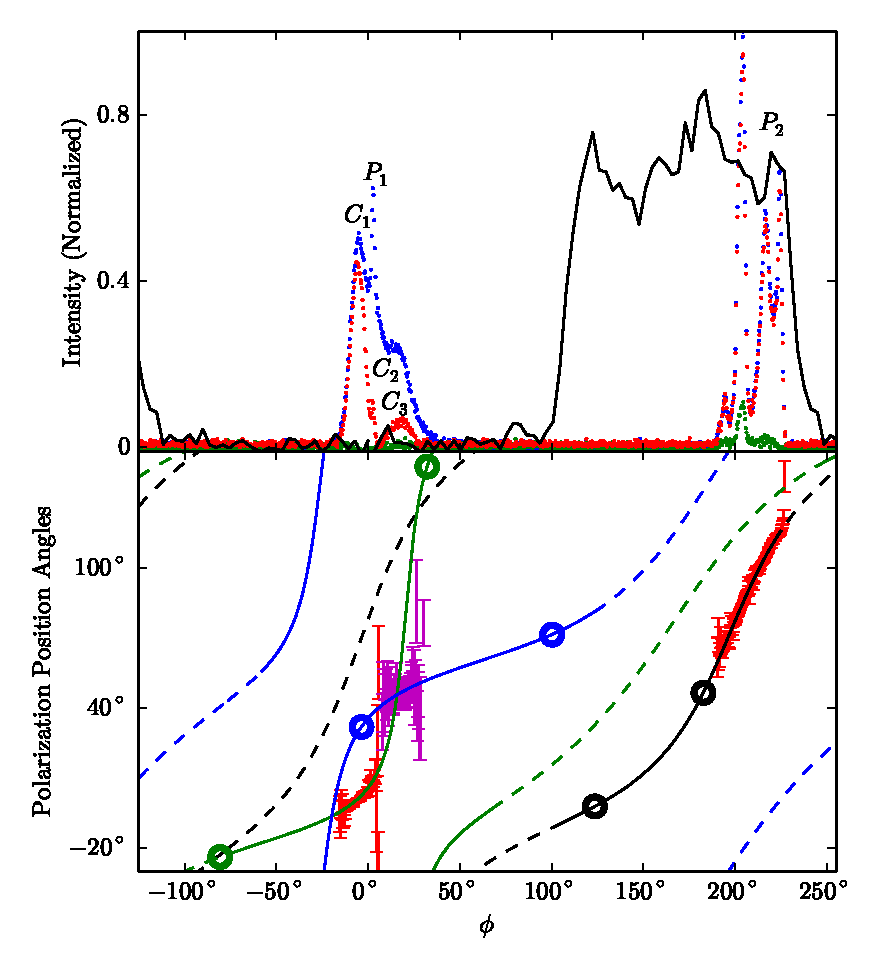
\includegraphics[scale=.8]{chapters/inwardDirectedPhotons/figures/intAndPAJ1057alpha77zeta50V2.eps}
\caption[ Intensity and polarization data for PSR J1057$-$5226 overlaid with bidirectional model]{\label{fig:singleAlt}
In the upper panel, blue points are total radio intensity 
data for 1.5GHz, red points are linear polarization intensity data
and green points are circular polarization intensity data for 
PSR J1057$-$5226.  Black solid line is $\gamma$-ray light
curve for emission greater than 0.1 GeV.
In the bottom panel, red data points with error bars are polarization position angles
in the outward-directed photon emission component (and RVM fit). The magenta data points with error bars are polarization 
position angles included in the inward-directed photon emission component, $P_{2}$.
The model polarization comes from
a fit with (unreduced) $\chi^2=419$ and parameters $\alpha=77^{\circ}$, $\zeta=48^{\circ}$,
and $R_{C_1/C_2}=R_{C_3}=R_{P_2}=0.35R_{\rm{LC}}$.  
The green and black lines are the model polarization for
outward-directed photon emission but from opposite poles.  
The blue line is the model
polarization of an inward-directed photon emission component
from the same pole as the black line. 
Empty circles mark limiting phase of emission from
open field lines with $\rho_{\rm{ypt}}=1R_{\rm{LC}}$.
Solid lines mark allowed emission phase for an effective open zone with
$\rho_{\rm{ypt}}=0.45R_{\rm{LC}}$ which is required for the model 
phase to cover all of the emission phase in the data.
Phase of zero is the point
of closest encounter to the magnetic axis in the model.
}
\end{center}
\vskip -.6truecm
\end{figure*}


\begin{figure}[htbp]
\begin{center}
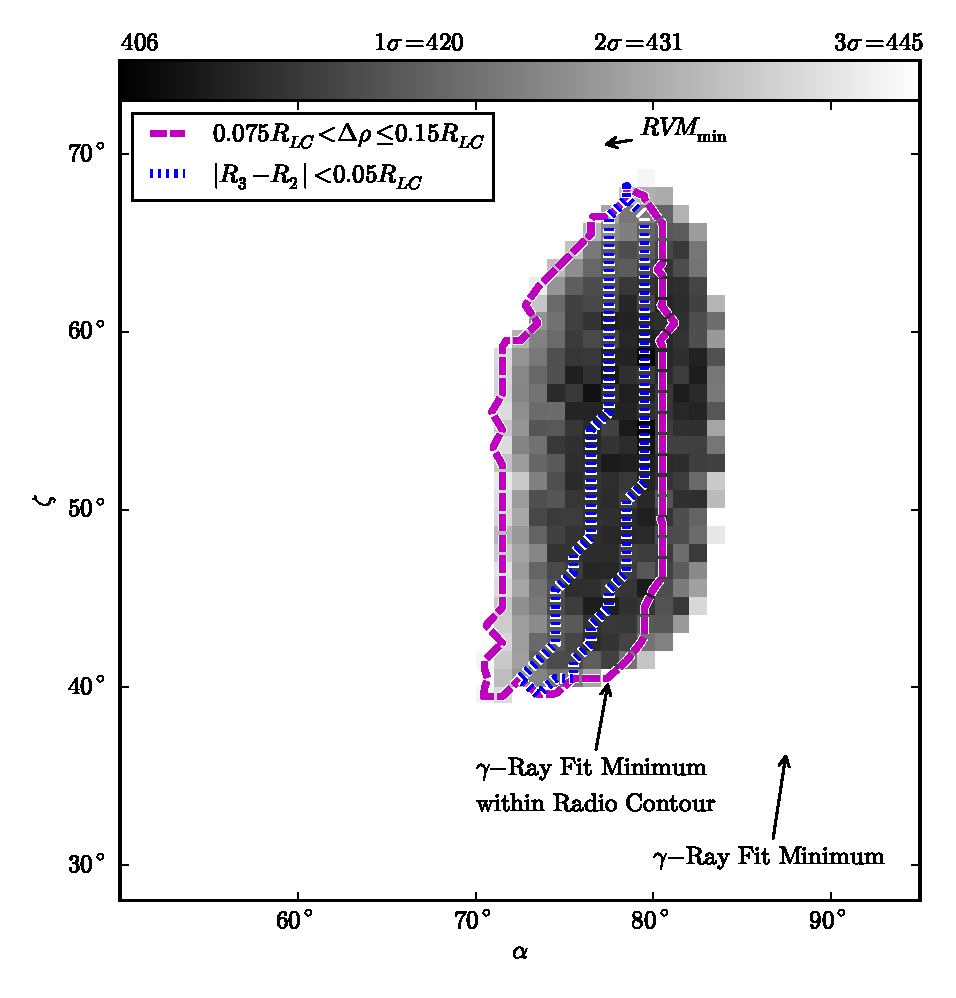
\includegraphics[scale=1]{chapters/inwardDirectedPhotons/figures/J1057-5226Map.eps}
\caption[Map of (unreduced) $\chi^2$ in the $\alpha$-$\zeta$ plane
for a three-altitude bidirectional fit to the polarization data of PSR J1057$-$5226]{\label{fig:map3}
Map of (unreduced) $\chi^2$ in the $\alpha$-$\zeta$ plane
for a three-altitude fit to the polarization data of PSR J1057$-$5226.
Blue contour shows the $3\sigma$ region above $\chi^2_{\rm{min}}$
for emission from the same pole (one outward-directed and one inward-directed)
with similar altitudes ($R_{C_3}$ and $R_{P_2}$).  The magenta contour shows 
the $3\sigma$ region above $\chi^2_{\rm{min}}$ for largest $\Delta \rho$ 
(the cylindrical distance from the largest emission distance to $\rho_{\rm{ypt}}$).
}
\end{center}
\vskip -.3truecm
\end{figure}


\begin{figure}[htbp]
\begin{center}
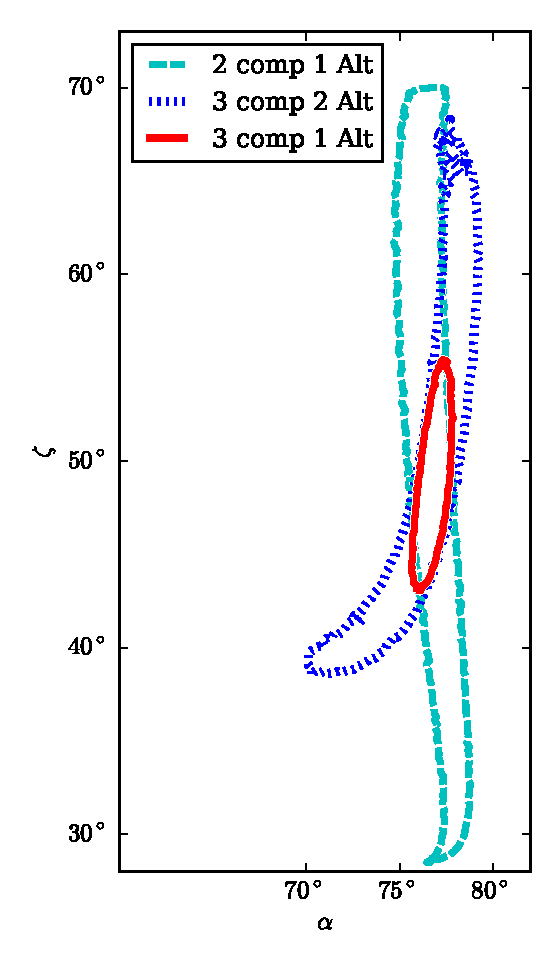
\includegraphics[scale=1]{chapters/inwardDirectedPhotons/figures/J1057-5226Map323.eps}
\caption[Map of (unreduced) $\chi^2$ in the $\alpha$-$\zeta$ plane
for a three-altitude fit to the polarization data of PSR J1057$-$5226]{\label{fig:c2}
Contours of $3\sigma$ region above $\chi^2_{\rm{min}}$ for three different fits
to the polarization data for PSR J1057$-$5226 in the $\alpha$-$\zeta$
plane. Cyan contour is the $3\sigma$ contour for fitting
the two outward-directed photon emission components (red data points with error bars only,
as seen in Figure~\ref{fig:totDirFitPhi}) with a single altitude ($R_{C_1/C_2}=R_{P_2}$).
The blue contour is the $3\sigma$ contour for the fit with both the two outward-directed
photon emission components and the one inward-directed photon emission component
with a single altitude for $C_1/C_2$ components and another for 
the $C_3$ and $P_2$ components as labeled on Figure~\ref{fig:totDirFitPhi} 
($R_{C_3}=R_{P_2}$).  The red contour is the $3\sigma$ contour
for a single-altitude fit such that $R_{C_1/C_2}=R_{C_3}=R_{P_2}$ with 
inward-directed photon emission for 
component $C_3$.  By assuming
a single altitude, allowed parameter space is strongly constrained.
Even with a two-altitude fit, $\alpha$ is strongly constrained.
}
\end{center}
\vskip -.3truecm
\end{figure}


\begin{table*}[t!!]
\caption{Fit parameters for PSR J1057$-$5226 (Bidirectional Emission)}
\tabcolsep=0.05cm
\begin{center}
\def\arraystretch{2}
\scalebox{0.83}{
\begin{tabular}{lccccccc}
\hline
\hline
& DOF&(unreduced) $\chi^2_{\rm{min}}$ & $\alpha$ ($^\circ$) & $\zeta$ ($^\circ$) & $R_{C_1/C_2}$ ($R_{\rm{LC}}$)& $R_{C_3}$ ($R_{\rm{LC}}$)&  $R_{P_2}$ ($R_{\rm{LC}}$)\\
[.3em] \hline

3 Alt& $228-7$ & $406$ & $76 ^{+7(+7)}_{-3(-6)}$ & $44 ^{+21(+24)}_{-3(-5)}$ & $0.40 ^{+0.06(+0.08)}_{-0.21(-0.28)}$ & $0.47 ^{+0.15(+0.21)}_{-0.36(-0.41)}$ & $0.44^{+0.07(+0.17)}_{-0.35(-0.38)}$  \\ \hline
2 Alt& $228-6$ & $   410 $ & $   77.4 ^{+1.2(1.6)}_{-4.6(-7.4)} $ & $52.4 ^{+12.4(+15)}_{-12.2(-13.8)} $ & $0.34 ^{+0.07(+0.09)}_{-0.14(-0.18)} $ & $0.32 ^{+0.19(+0.25)}_{-0.17(-0.20)} $ &  \\ \hline
1 Alt& $228-5$ & $   419 $ & $   76.6 ^{+0.8(+1.2)}_{-0.6(-1.0)} $ & $47.6 ^{+5.4(+8.2)}_{-3.6(-4.8)} $ & $ 0.35 ^{+0.05(+0.07)}_{-0.02(-0.03)} $ &  & \\ \hline



\end{tabular}}
\tablecomments{ Errors reported without (with) parentheses are for $1\sigma$ ($3\sigma$) from $\chi^2_{\rm{min}}$.}
\label{tb:fit}
\end{center}
\end{table*}





\begin{table*}[t!!]
\caption{Measured Parameters for PSR J1057$-$5226 (Bidirectional Emission)  }
\begin{center}
\begin{tabular}{llll}
\hline
&$\Delta \rho$ ($R_{\rm{LC}}$)& $\rho_{\rm{max}}$ ($R_{\rm{LC}}$)& $\rho_{\rm{ypt}}$ ($R_{\rm{LC}}$)\\
\hline & \\[-1em]\hline

3 Alt&$0.12^{+0.02(+0.02)}_{-0.12(-0.12)}$ & $0.39^{+0.08(+0.16)}_{-0.21(-0.26)}$ & $0.51^{+0.07(+0.14)}_{-0.35(-0.48)}$  \\ \hline
2 Alt&$0.12^{+0.01(+0.02)}_{-0.05(-0.06)}$ & $0.29^{+0.16(+0.22)}_{-0.11(-0.15)}$ & $0.41^{+0.17(+0.23)}_{-0.15(-0.16)}$  \\ \hline
1 Alt&$0.12^{+0.01(+0.01)}_{-0.01(-0.01)}$ & $0.34^{+0.02(+0.03)}_{-0.03(-0.05)}$ & $0.46^{+0.02(+0.03)}_{-0.03(-0.05)}$  \\ \hline

\end{tabular}
\tablecomments{Errors reported without (with) parentheses are for $1\sigma$ ($3\sigma$) from $\chi^2_{\rm{min}}$.}
\label{tb:meas}
\end{center}
\end{table*}

In Figure~\ref{fig:singleAlt}, the best fit single-altitude
model overlays the polarization data of PSR J1057$-$5226. 
Red data points match well to 
outward-directed photon model polarization.  This polarization (outward only)
also matches reasonable well to the RVM model, $\chi^2=325$ (unreduced, Degrees of Freedom $=\rm{DOF}=166-4$).
The best fit RVM model is labeled on Figure~\ref{fig:map3}.
The RVM fit is problematic because it requires emission
from well within the closed zone of the pulsar magnetosphere
\citep{weltevrede2009mapping}.  \cite{craig2014tackling}  fit the red points (in Figure~\ref{fig:singleAlt})
with a finite-altitude model and found even better
fits with altitudes either far from the neutron star or within
the closed zone and fits in between these extremes.  Unfortunately, this model
was unable to model the data points in magenta. 
In the current paper, 
we explored the possibility that 
the magenta points originate from inward-directed photon emission.

Figure~\ref{fig:map3} shows the (unreduced) $\chi^2$ surface in the $\alpha-\zeta$
plane for position angle data modeled using a three-altitude
model with inward-directed photon emission for component $C_3$.  The lowest (unreduced) $\chi^2$
was $406$ with $\rm{DOF}=228-7$.  Table \ref{tb:fit} shows best fit parameters
as well as $1\sigma$ and $3\sigma$ error bars for those parameters.  The blue contour
of Figure~\ref{fig:map3} is the $3\sigma$ from $\chi^2_{\rm{min}}$ contour for models with similar 
$R_{C_3}$ and $R_{P_2}$.  Since component $C_3$ and $P_2$ are from the same pole,
it is not unreasonable to assume they are from similar heights.  The magenta
contour is the $3\sigma$ from $\chi^2_{\rm{min}}$ contour of models with the 
largest $\Delta\rho$ (see Section \ref{sec:fitProcedure} for definitions).  Models with larger $\Delta\rho$ 
are more trustworthy since field lines close to the y-point will be
distorted in manners not accounted for in our vacuum dipole model.  The
component $P_2$ drives this parameter to such small values while components $C_1/C_2$
and $C_3$ for the most part originate well away from the y-point cylindrical distance.
Figure~\ref{fig:singleAlt} illustrates this point well.
Empty circles on the figure mark the expected phase of emission for the 
classical dipole open zone ($\rho_{\rm{ypt}}=1R_{\rm{LC}}$).  For
this particular set of fit parameters $C_1/C_2$ and $C_3$
data are both well within the classical open zone while
$P_2$ data is entirely outside of this phase range.

Figure~\ref{fig:c2} shows the $3\sigma$ from $\chi^2_{\rm{min}}$ contour in the $\alpha-\zeta$
plane of a variety of fitting schemes.  The cyan contour is the $3\sigma$ area 
in the $\alpha-\zeta$ plane of a fit done with only $C_1/C_2$ and $P_2$ data and a single
altitude.  These are the outward-directed photon emission components.  The blue contour represents
the fit with all three components but with different altitudes for the 
different poles ($C_3$ and $P_2$ have the same altitude, similar to the blue
contour on Figure~\ref{fig:map3}).  The fit
represented with the blue and cyan contours both have large ranges
of acceptable $\zeta$.  The red contour is the $3\sigma$ from
$\chi^2_{\rm{min}}$ area for a fit with a single altitude, $R_{C_1/C_2}=R_{C_3}=R_{P_2}$.
Not surprisingly, this is roughly the overlap of the cyan and blue contours.
Further, unlike the blue and cyan contours, the red contour (representing the assumption
of a single altitude) greatly restricts the possible $\zeta$ range.

Table \ref{tb:fit} compares fit parameters assuming one,
two, and three altitudes.  $\chi^2_{\rm{min}}$ did not drastically change
by adding new free parameters (additional altitudes) nor did
the best fit parameters shift drastically.  
Table \ref{tb:meas} shows parameters that can be measured
from the model fitting.  Again these measured parameters remain the
same for different numbers of altitudes although
the allowed range of the parameters decreases with
fewer fit altitudes.

\subsubsection{Fitting PSR J1057$-$5226 with Outward-Directed Photon Emission}
\label{sec:outwardOnly}
We will briefly discuss fit results of simulations with 
only outward-directed photon emission.  We 
fit with a three-altitude model assuming that
the emission for $C_1/C_2$, $C_3$, and $P_2$
all originated from photons directed away from the
neutron star center.
The lowest (unreduced) $\chi^2_{\rm{min}}=435$ ($\rm{DOF}=228-7$).
For this fit, $\alpha=79^\circ$, $\zeta=35^\circ$, $R_{C_1/C_2}=.54R_{\rm{LC}}$, $R_{C_3}=.86R_{\rm{LC}}$,
and $R_{P_2}=.5R_{\rm{LC}}$.  The $\chi^2_{\rm{min}}$ is just inside
the $3\sigma$ contours of the three-altitude fit assuming
an inward-directed photon emission component; the $\chi^2$
increases significantly within a couple of degrees of this $\chi^2_{\rm{min}}$
at $\alpha=79^\circ$, $\zeta=35^\circ$.
Statistically, the bidirectional model is
better suited to the data over a larger region of 
parameter space and it is visually more satisfying.

\subsubsection{Visualizing the Pulsar Configuration}
\label{sec:config}


Figure~\ref{fig:totDirFitPhi} shows one possible configuration
of the pulsar with inward-directed photon emission for component $C_3$
and that produces position angle polarization sweeps similar
to the data (see Section \ref{sec:fitProcedure} for more
details on the fitting procedure).  This particular configuration
produces the best fit $\chi^2$ assuming emission
from a single altitude ($R_{C_1/C_2}=R_{C_3}=R_{P_2}$).

In the figure, the yellow field lines are 
last closed field lines with $\rho_{\rm{ypt}}=1R_{\rm{LC}}$,
and the cyan field lines are those with $\rho_{\rm{ypt}}=0.45R_{\rm{LC}}$.
For all emission from the $P_2$ component to originate
from open field lines, $\rho_{\rm{ypt}}=0.45R_{\rm{LC}}$.  The grey areas in 
Figure~\ref{fig:totDirFitPhi} are the open field line 
caps at an altitude of $0.35R_{\rm{LC}}$ and $\rho_{\rm{ypt}}=0.45R_{\rm{LC}}$.
The black lines on the caps are the boundary of the caps if 
$\rho_{\rm{ypt}}=1R_{\rm{LC}}$.  Note that the yellow field lines
touch the black line boundary while the 
cyan field lines touch the grey cap boundary.

The red curves on the caps indicate the 
emission locations visible at $\zeta=48^\circ$.  Thicker (curved)
red lines indicate regions of signal in the data for this
given configuration (see Figure~\ref{fig:singleAlt}). 
The thick (curved) red line for $P_2$ goes to the
edge of the grey cap; as discussed earlier, $P_2$
is the component that controls $\rho_{\rm{ypt}}$.
The large phase of emission
requires a low $\rho_{\rm{ypt}}$ or a high altitude
to accommodate the 
$P_2$ emission.  In previous fitting that included only 
polarization data from $C_1/C_2$ and $P_2$, we
could find a few solutions with $\rho_{\rm{ypt}}=1R_{\rm{LC}}$
(the classical dipole open cone of emission) 
within the $3\sigma$ contour from $\chi^2_{\rm{min}}$;
but with the addition of fitting $C_3$ data,
these fits are no longer probable.  

Green arrows from the curves indicate the direction of emission.
The arrow from $C_3$ emission goes into the pulsar magnetosphere.
Locations of $C_3$ and $P_2$ emission are on opposite sides of the same pole.
This is necessary geometrically in order for the inward-directed and
outward-directed photon emission to be visible from the same $\zeta$.

\subsection{Combining $\gamma$-Ray Fitting with Radio Polarization Model}
\label{sec:gam}
One striking feature of the PSR J$1057-5226$ $\gamma$-ray data is the overlap in phase
with the radio data.  
The upper panel of Figure~\ref{fig:singleAlt} shows
the $\gamma$-ray light curve in black over the radio emission.  The 
$\gamma$-ray light curve lines up with the $P_2$ pulse suggesting that
both could be coming from similar locations in the magnetosphere.  
This is an unusual feature for pulsar emission and may give evidence to 
the seemingly unusual emission from the $P_2$ component.

\subsubsection{$\gamma$-Ray Model Method}
%gamma and radio come from same place

The $\gamma$-ray
data was obtained from the \textit{Fermi} LAT pulsar catalog (\citealp{abdo2010fermi,abdo2013second}).
The data is from energies greater than $0.1$ GeV.
The $\gamma$-ray model is based on \cite{romani2010constraining}.  
The outer gap model
has emission originating from inside the effective light cylinder ($\rho_{\rm{ypt}}$)
and beyond the null charge surface ($\vec{B}\cdot\vec{\Omega}=0$).  We use the same emissivity function 
($e^{-[(s-2 s_{\rm{NC,min}}-1)/0.1]^2}$ for beyond a path length of $1+2 s_{\rm{NC,min}}$ and constant below, where 
$s$ is the path length, $s_{\rm{NC,min}}$ is the minimum path length of field lines at a given fraction of the polar cap, and
units are in terms of $R_{\rm{LC}}$) as \cite{romani2010constraining}.
Emission was allowed for a range of effective $w$ values
from $.01$ to $.12$ where $w$ is the fraction of the radial distance
from the pole on the polar cap.  Here we use an ``effective''
$w$ in that the polar cap defined by the open field lines will shift
based on $\rho_{\rm{ypt}}$.  A Gaussian width was applied to a given $w$ 
slice of $0.02$ (again similar to \citealp{romani2010constraining}).

\subsubsection{$\gamma$-Ray Model Results}

\begin{figure}[t!!]
\begin{center}
\includegraphics[scale=.7]{chapters/inwardDirectedPhotons/figures/plotBestFits.ps}
\caption[Data and best models for $\gamma$-ray light curve of PSR J1057$-$5226]{\label{fig:gammaBestFits}
Black data points with error bars are $\gamma$-ray data for energy greater than $0.1$ GeV.
The magenta line is the best fit $\gamma$-ray light curve using extrapolated 
parameters.  The green line is the best fit $\gamma$-ray light curve using
parameters only within the $3\sigma$ from $\chi^2_{\rm{min}}$
space of the radio fit results.  The cyan line is the
best fit $\gamma$-ray light curve using the parameters at the 
best radio fit for a single-altitude model.}
\end{center}
\vskip -.4truecm
\end{figure}


\begin{figure}[t!!]
\begin{center}
\includegraphics[scale=.7]{chapters/inwardDirectedPhotons/figures/plotCombinedw60w150.ps}
\caption[Data and variable $w$ model for $\gamma$-ray light curve of PSR J1057$-$5226]{\label{fig:gammaCombinedw60w150}
Black data points with error bars are $\gamma$-ray data for energy greater than $0.1$ GeV.
The blue line and red line are $\gamma$-ray light curves using the parameters at the 
best radio fit for a single-altitude model and $w=0.15$ and $w=0.06$.
The magenta line is a $\gamma$-ray light curve from a model that illuminates 
field lines between $w=0.15$ and $w=0.06$ from one end of the light curve to the other.
This model illustrates that better model light curves are possible in regions of 
the best fit radio models but they would require modifications to 
the prescription of illuminated field lines.
}
\end{center}
\vskip -.4truecm
\end{figure}



We limited our parameter space to $\alpha$, $\zeta$, $\Delta \phi$, and
$\rho_{\rm{ypt}}$ within $3\sigma$ of the $\chi^2_{\rm{min}}$
of the radio modeling results.  Additionally,
$\rho_{\rm{ypt}}$ obtained in the radio polarization fitting is
an \textit{upper} limit and the lower limit is set by 
the geometrical location of the radio emission
with the largest cylindrical distance from the spin axis.
We focused on fitting with only maximum $\rho_{\rm{ypt}}$ since smaller
y-point distances revert the model to essentially a simple
dipole.  This in turn eliminates the caustics and box-like
sides of the emission which are clearly seen in the data 
(see Figures~\ref{fig:gammaBestFits} and \ref{fig:gammaCombinedw60w150} for data).
In general, models with smaller $\rho_{\rm{ypt}}$ yield
worse fits because of this.  Further, fits with  larger
$\zeta$ ($\gtrsim 55^\circ$) tended to have smaller
required $\rho_{\rm{ypt}}$ (from radio fits) and 
poorer $\chi^2$ values due to this.

With this relatively simple $\gamma$-ray model
and the radio fit restrictions, the best fit model is
$\alpha=77^\circ$, $\zeta=40^\circ$, $w=0.04$, with unreduced $\chi^2_{\rm{min}}=695$.
The degrees of freedom for the $\gamma$-ray fits are $\rm{DOF}=100-1$ since
only $w$ is being fit.
Here the $\chi^2_{\rm{min}}$ in radio is 445 right at the $3\sigma$
cut off of the fits.  



Admittedly, the $\gamma$-ray model is not
exact, neglecting important plasma physics that can
affect the field line structure, particularly at
high altitudes, in addition to making simplistic 
assumptions about $\gamma$-ray production locations.  Further, having the minimum 
$\chi^2$ region for the $\gamma$-ray model close to the minimum
in polarization is encouraging even if they do not
exactly overlap and still indicates some real features are
being captured by the model.
Since the minimum $\chi^2$ of the $\gamma$-ray model is right at the 
3$\sigma$ edge of the $\chi^2$ surface of the radio polarization fit, we are interested in
the behavior of the $\gamma$-ray model beyond this region.
Calculating $\chi^2$ values of the $\gamma$-ray model
using radio fit model values is not sensible since radio models beyond $3\sigma$
do not contain real information and are poor matches to the data.
Instead, we expanded the allowed region
around this fit space for the radio model within $3\sigma$ 
of $\chi^2_{\rm{min}}$by extrapolating parameters using simple piece-wise
linear fitting. 

The lowest local unreduced $\chi^2$
is 322 with $\alpha=87^\circ$, $\zeta=36^\circ$, $w=0.02$ 
for fits in the extrapolated region.
Decreasing $\zeta$ further resulted in the worsening of $\chi^2$.
Unfortunately the unreduced $\chi^2$ for the radio is 3400, far beyond what 
would be statistically acceptable and visually unsatisfactory.  

On Figure~\ref{fig:map3} is a marking for the lowest $\chi^2$ from the $\gamma$-ray 
fitting both within the $3\sigma$ radio fit contour and 
without the contour. Ideally, the best fit $\gamma$-ray model would fall
within the best fit parameter space of the polarization radio model.
But considering the uncertainties of the $\gamma$-ray model,
the lowest local $\gamma$-ray $\chi^2$ is not
dramatically far from $\chi^2$ minimum area of the 
radio polarization fit.   
From this information we can conclude that a joint
fit between radio and $\gamma$-ray data would fall around $\zeta\sim40^\circ$.

Figure~\ref{fig:gammaBestFits} shows the best fit light curves
for within the $3\sigma$ contour of the radio results (green)
and the local minimum fit in the $\gamma$-ray just 
beyond this contour (magenta).  Both appear relatively 
flat compared to the data.  Also plotted in the same figure 
in cyan is the best fit light curve at $\alpha=77^\circ$, $\zeta=48^\circ$ 
(unreduced $\chi^2=5000$, $\rm{DOF}=100-1$),
the best fit values in the radio polarization for the single-altitude model. The model light curves are normalized to the total 
counts.

The \textit{position} of the pulse
using this $\gamma$-ray model 
matches the light curve position; the morphology of the 
peaks within the pulse are not matched. 
If $w$ is not constant, models much more suited for the single-altitude
polarization fit space in terms of pulse width are obtainable.  
Whether this would improve the morphology is unclear but 
certainly possible.
At the moment, a prescription
for a $w$ that is variable is unclear.

To illustrate this point, we produced a 
light curve which varied between $w=0.06$ and $w=0.15$
(linearly with respect to magnetic $\phi$).  This
light curve is plotted in Figure~\ref{fig:gammaCombinedw60w150}
over the data.  
The curve is not fit to the data but is meant simply 
as an illustration; undoubtedly, using a different prescription
for field line illumination or slightly different $\alpha$ and $\zeta$
could result in better fits to the data in the $3\sigma$ parameters
space of the radio data.  But without a
clear and physically motivated prescription, any curves would be 
purely ungrounded speculation.
Also plotted in Figure~\ref{fig:gammaCombinedw60w150}
are light curves with constant $w=0.06$ (solid, red) and $w=0.15$ (dashed, blue).

We can therefore conclude that the $\gamma$-ray 
fitting favors smaller $\zeta$ but perhaps not quite
as strongly as may be suggested by models where field lines
of a single $w$ are illuminated.  Either way, results suggest a lower $\zeta$
than that of RVM ($\alpha=77^\circ$, $\zeta=70^\circ$, ignoring the $C_3$ component) 
which is consistent with bidirectional, finite-altitude radio polarization fitting. 

\subsection{Discussion and Conclusions}
\label{sec:conclusions}

\subsubsection{Comparison to \cite{weltevrede2007main}}

The bidirectional model of PSR J1057$-$5226 presented in \cite{weltevrede2007main} 
(Figure 12) is different from the one presented in
the current paper.  The configuration for PSR J1057$-$5226 is very similar to
the one given for PSR B1702$-$19 in the same paper.  Our particular
configuration was motivated by the shape of the polarization curve while
the configuration of \cite{weltevrede2007main} was motivated by modulations
in the intensity.  First, the model of \cite{weltevrede2007main} Figure 12
divides the emission of the pulse $P_2$ into a modulated and an
unmodulated component.  The paper \cite{weltevrede2012phase} does support
$P_2$ having several different modulations among the peaks.  Yet the
polarization of $P_2$ is smooth and connected between the various
components and thus the emission is very likely to come from the same
location in the magnetosphere.  Second, the model of \cite{weltevrede2007main} 
has the emission from the pulse we label as $P_1$ from a single
location in the magnetosphere whereas in the model presented here
the $P_1$ pulse is split into outward-directed photon emission and
inward-directed photon emission.  The motivation here was again driven
by the polarization sweep.  A clear disconnect exists between the
polarization of components $C_1/C_2$ and the component $C_3$.  Considering these two pieces of
polarization are from the same pole, whether the emission was from
outward-directed photons (as discussed in Section \ref{sec:outwardOnly}) or from
inward-directed photons (with and without multiple altitudes and
orthogonal mode jumps), did not yield appropriate models.  The best fit
model with the pulse $P_1$ emitted wholly from inward-directed photons and
$P_2$ emitted from outward-directed photons had an unreduced $\chi^2$ of $786$.  

On the other hand, the polarization of $C_1/C_2$ and $P_2$ are well-defined with
small error bars while the polarization of $C_3$ has
larger error bars and is generally more noisy.  It is
then natural to assume that the emission of $C_1/C_2$ and $P_2$ is typical,
outward-directed photon emission and the emission of $C_3$ is unusual.
Further, the emission of component $C_3$ is located after the phase of
emission of components $C_1/C_2$, the location where emission from
inward-directed photons of the opposite pole would appear.  Thus the
model configuration used in this paper was a natural choice before any
formal fitting was performed.


\subsubsection{Comparison to \cite{weltevrede2009mapping}}

As noted earlier, \cite{weltevrede2009mapping} analyzed polarization data of
PSR J1057$-$5226.  They use the RVM to calculate polarization sweeps.
The magnetic field lines are simple vacuum dipole (RVM) but they included
retardation and aberration effects to calculate the height estimations
from BCW. In addition, they use pulse width arguments to calculate emission 
height.  They estimate the
altitude of emission from both poles  is $0.07R_{\rm{LC}}$.  At this altitude, the
polarization sweeps will not be drastically distorted \citep{craig2012altitude} 
and RVM is appropriate to use assuming this altitude.  Also at this altitude, the
magnetic field lines in the numerical model will be essentially the same
as RVM.  Further, at low altitudes, polarization position angles for
inward-directed photons and outward-directed photons will be similar.
The polarization of VII as labeled in \cite{weltevrede2009mapping}
(corresponding to $C_3$ in the current paper) is unlikely to have strongly
influenced the RVM polarization fitting since there are few data points
for $C_3$ and these data points have larger error bars compared to the rest
of the polarization sweep (as can be noted from Figure 2 of \citealp{weltevrede2009mapping}).  
With these considerations and if the numerical model used
in the current paper were applied to the data of \cite{weltevrede2009mapping}
with a low altitude constraint, the polar cap map of Figure 7 in
\cite{weltevrede2009mapping} would be similar.  The difference would be that
the VII line section (the inward-directed photon emission) would be
located in the upper left quadrant and on the same pole as the
I-II-III-IV line section of the diagram.

In \cite{weltevrede2009mapping}, they describe the last closed field lines
needed for the emission to originate from open field lines in terms of a
footprint parameter.  This footprint parameter is a measure of the cap
size on the neutron star surface.   In addition, for their favored
configuration, they state that the last closed field line closes at a distance
of a quarter of a light cylinder radius (e.g. $\rho_{\rm{ypt}}=0.25R_{\rm{LC}}$).  For our best
fit single-altitude models $\rho_{\rm{ypt}}\sim0.46R_{\rm{LC}}$ and $R\sim0.35R_{\rm{LC}}$.  The favored
altitude of  \cite{weltevrede2009mapping} is $0.07R_{\rm{LC}}$.  Roughly, the model
presented here is a natural extension of the \cite{weltevrede2009mapping}
model that allows larger finite altitude.  Because our model allows
larger altitudes, the needed $\rho_{\rm{ypt}}$ is consistently higher.  Our $\Delta \rho_{\rm{ypt}}$
(the cylindrical distance between the maximum emission distance and the
effective light cylinder) is $\sim0.12R_{\rm{LC}}$.  For \cite{weltevrede2009mapping}, we
can estimate $\Delta \rho_{\rm{ypt}}$ as $0.25-0.07=0.18R_{\rm{LC}}$ which again is roughly
consistent with the numerical model.

\subsubsection{Comparison to \cite{weltevrede2012phase}}
\label{sec:comp2012}
In \cite{weltevrede2007main}, the authors argued for a bidirectional model
for PSR B1702$-$19 based on phase locked modulation and include a schematic 
of a possible PSR J1057$-$5226
bidirectional model.  However, in \cite{weltevrede2012phase}, bidirectional
emission models are avoided presumably because 
the phase locked modulation delay is too large
for the simple time of flight delay for bidirectional emission
from the same location in the magnetosphere.  The
model relies on emission from the exact same location in the
magnetosphere for both
inward-directed and outward-directed photons.  
For our model, the emission is from the same pole but on
opposite sides of the pole.  Thus a
larger difference in modulation delay time
may not be reasonable.

Further, the modulation reported in \cite{weltevrede2012phase} are present
mostly in the peaks we label as $C_1$ and $C_2$.  These peaks (labeled as V
and VI in \citealp{weltevrede2012phase}) are modeled as forward-directed photon
emission.  The trailing edge of the pulse (mostly the peak labeled as $C_3$
in the current paper and VII in \citealp{weltevrede2012phase}) does not
participate in the $2.5P$ modulation.  If the phase-locked modulation was
connected to the bidirectional emission model presented here, the peak
$C_3$ (modeled as originating from the inward-directed photons) should
modulate with the $P_2$ peak.

Finally, the modulation in $C_1$ and $C_2$ and the lack of modulation in $C_3$
indicates that $C_1$ and $C_2$ are distinct from $C_3$.  This supports the
bidirectional model since $C_1$ and $C_2$ come from the opposite pole compared
to $C_3$.  In this model we would not expect emission from these different
peaks to modulate with one another.


\subsubsection{Summary}
The position angle polarization data for PSR J1057$-$5226 is inconsistent with
the typical geometrically-based polarization model, RVM.  Based
on the data, RVM was modified to include orthogonal mode
jumps, multiple finite altitude, and bidirectional emission.
With these modifications, the produced
polarization position angle sweeps are consistent with the data.  
Assuming a single altitude of emission greatly
restricts the acceptable parameter space. 
The data still requires the
y-point further in than the classical
light cylinder distance but this atypical behavior may 
lend hints to the bidirectional nature of PSR J1057$-$5226.


Further, $\gamma$-ray modeling with a model of the simplest outer gap
formulation is possible.  The $\gamma$-ray models favor the smallest $\zeta$
values when restricted 
by radio model fitting parameters within
$3\sigma$ of $\chi^2_{\rm{min}}$.
These models do capture the overall shape of the pulse but a more precise fit
will likely required better understanding of the location of the $\gamma$-ray
emission.   Additionally, in our current model, we neglect plasma effects which
might be important at the altitudes that are modeled here.  Further,
PSR J1057$-$5226 has unusual modulation patterns in its intensity.  Surely, these
modulation hold tantalizing keys to the pulsar emission and indicate
atypical behavior; yet we are unable to incorporate these modulations in our
model.


In brief, bidirectional emission is consistent with both
radio and $\gamma$-ray data and is an
exciting possibility for the unusual emission
of the pulsar PSR J1057$-$5226.


\acknowledgements
We greatly thank S. Johnston for supplying radio data for PSR J1057$-$5226 (2012, private correspondence)
and Roger W. Romani for valuable discussion. This work has been 
supported by the Stanford Office of
the Vice Provost of Graduate Education DARE Doctoral
Fellowship Program to H.A.C.


